
\section{Quelques structures de données}
\subsection{Les enregistrements}

\begin{frame}
	\begin{center}
		\huge 
		Les structures de données
	\end{center}
\end{frame}


\begin{frame}[fragile]
	\frametitle{Enregistrements}
	\begin{itemize}
	\item Déclaration de type: 
		\begin{lstlisting}
		  type pixel = 
		  { 
		     mutable r:float; 
		     mutable g:string; 
		     b:int;
		  } 
		
		let p = { r=2.4; g="The Game"; b=255 }
		\end{lstlisting}
	\item Accès et modification des champs de valeur:
		\begin{lstlisting}
			  p.b;;
			  -: int = 255
			  p.g <- "You Lose"
		\end{lstlisting}
	\end{itemize}
\end{frame}


\begin{frame}[fragile]
	\frametitle{Les références}
	Une référence est considérée comme l'équivalent (selon l'INRIA) des pointeurs en OCaml.\\
	Déclaration:
	\begin{lstlisting}
		  let a = ref 0

	\end{lstlisting}
	Utilisation:
	\begin{lstlisting}
		  !a ;;
		  - : int = 0
		  a := !a + 1 ;;
		  - : unit = ()
	\end{lstlisting}

\end{frame}

\subsection{Les vecteurs}

\begin{frame}
	\frametitle{Les vecteurs}
	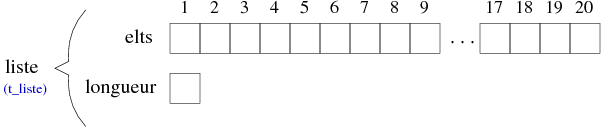
\includegraphics[scale=0.5]{pics/vect.png}
\end{frame}

\begin{frame}[fragile]
	\frametitle{Les vecteurs}
	\framesubtitle{Création}
	\begin{itemize}
	\item
	\begin{lstlisting}
	let v = [| 3.14; 6.28; 9.42 |];;
	val v : float array = [|3.14; 6.28; 9.42|]
	\end{lstlisting}

	\item Array.make
	\begin{lstlisting}
	let v = Array.make  3  3.14;;
	val v : float array = [|3.14; 3.14; 3.14|]
	\end{lstlisting}

	\end{itemize}
\end{frame}


\begin{frame}[fragile]
	\frametitle{Les vecteurs}
	\framesubtitle{Utilisation simple}
	\begin{itemize}
	\item
	\begin{lstlisting}
	v ;;
	- : float array = [|100; 3.14; 3.14|]
	\end{lstlisting}

	\item
	\begin{lstlisting}
	v.(1) ;;
	- : float = 3.14
	\end{lstlisting}

	\item
	\begin{lstlisting}
	v.(0) <- 100.0 ;;
	- : unit = ()
	\end{lstlisting}
	\end{itemize}
\end{frame}

\begin{frame}[fragile]
	\frametitle{Les vecteurs}
	\framesubtitle{Copie et valeurs partagées}
	\begin{block}{Soit une copie simple}
	\begin{lstlisting}
	let v = Array.make 3 1;;
	val v : int array = [|1; 1; 1|]
	let m = Array.copy v ;;
	val m : int array = [|1; 1; 1|]

	v.(1)<- 1337;;
	- : unit = ()

	m;;
	-: int array = [|1; 1; 1|]
	\end{lstlisting}
	\end{block}
\end{frame}

\begin{frame}[fragile]
	\frametitle{Les vecteurs}
	\framesubtitle{Autres fonctionnalitées du module Array}
	\begin{itemize}
	\item Array.make\_matrix
	
	\item Array.iter

	\item Array.map 

	\item Array.iteri

	\item Array.to\_list

	\end{itemize}
\end{frame}

\subsection{Les piles}
\begin{frame}
	\frametitle{Les piles}
	
\includegraphics[scale=0.4]{pics/stack.jpg}
\end{frame}

\begin{frame}[fragile]
	\frametitle{Les piles}
	\framesubtitle{Initialisation}
	Pour utiliser les piles en OCaml nous vous présenterons ici le module Stack :
	\begin{lstlisting}
	open Stack
	\end{lstlisting}
	Pour créer une pile on utilise:
	\begin{lstlisting}
	let s = Stack.create ();;
	val s : '_a Stack.t = <abstr>
	\end{lstlisting}
\end{frame}

\begin{frame}[fragile]
\frametitle{Les piles}
\framesubtitle{Utilisation}
	\begin{itemize}
	
	\item
		\begin{lstlisting}
		Stack.push 42 s; Stack.push 1337 s;;
		- : unit = ()	
		\end{lstlisting}	
	
	\item
		\begin{lstlisting}
		Stack.pop s;;
		- : int = 1337
		Stack.top s;;
		- : int = 42
		\end{lstlisting}	

	\end{itemize}

\end{frame}

\begin{frame}[fragile]
	\frametitle{Les piles}
	\framesubtitle{Les fonctions essentielles}
	\begin{itemize}
	
	\item
		\begin{lstlisting}
		Stack.clear
		\end{lstlisting}

	\item
		\begin{lstlisting}
		Stack.copy
		\end{lstlisting}	

	\item
		\begin{lstlisting}
		Stack.is_empty
		\end{lstlisting}	

	\item
		\begin{lstlisting}
		Stack.length
		\end{lstlisting}	

	\item
		\begin{lstlisting}
		Stack.iter
		\end{lstlisting}

	\end{itemize}

\end{frame}

